%----Símbolos matemáticos definidos por ISO 80000-2:2009------------------------
\newcommand{\defeq}{\mathrel{\mathop:}=} %El signo de "igual por definición"
\let\gets\defeq
\newcommand{\transpose}[1]{{#1}^{\operatorname{T}}} %Operadores en letra derecha
\newcommand{\invert}[1]{{#1}^{-1}}
\newcommand{\bigOh}[1]{\operatorname{O}\left( #1 \right)}

\newcommand{\dist}[2]{\mathit{d}\left(#1 , #2\right)} %Excepto la distancia

\newcommand{\mat}[1]{\boldsymbol{#1}} %Las matrices van en negrita itálica
\renewcommand{\vec}[1]{\boldsymbol{#1}} %...y los vectores también
\newcommand{\entry}[3]{\left({#1}\right)_{{#2}\,{#3}}} %Entrada de una matriz
\newcommand{\sgn}{\operatorname{sgn}}
\newcommand{\abs}[1]{\left|{#1}\right|}

\newcommand{\Set}[1]{\left\{{#1}\right\}}
\newcommand{\Tuple}[1]{\left({#1}\right)}
\newcommand{\BuildSet}[2]{\left\{ #1 \middle| #2 \right\}}
\newcommand{\Nset}{\ensuremath{\mathbf{N}}} %Conjuntos numéricos en negrita
\newcommand{\Zset}{\ensuremath{\mathbf{Z}}}
\newcommand{\Rset}{\ensuremath{\mathbf{R}}}
\newcommand{\Cset}{\ensuremath{\mathbf{C}}}
\newcommand{\ident}{\ensuremath{\mat I}} %La matriz identidad se denota con I

\renewcommand{\leq}{\leqslant} %El símbolo menor-igual va inclinado
\renewcommand{\geq}{\geqslant} %...y también el mayor-igual
\let\le\leq
\let\ge\geq

%----Símbolos propios de este documento-----------------------------------------
\newcommand{\DynA}{\ensuremath{\mathbb{A}}} %Tipos Dynkin
\newcommand{\DynAtilde}{\ensuremath{\tilde{\mathbb{A}}}}
\newcommand{\DynB}{\ensuremath{\mathbb{B}}}
\newcommand{\DynC}{\ensuremath{\mathbb{C}}}
\newcommand{\DynD}{\ensuremath{\mathbb{D}}}
\newcommand{\DynDtilde}{\ensuremath{\tilde{\mathbb{D}}}}
\newcommand{\DynE}{\ensuremath{\mathbb{E}}}
\newcommand{\DynEtilde}{\ensuremath{\mathbb{E}}}
\newcommand{\DynF}{\ensuremath{\mathbb{F}}}
\newcommand{\DynG}{\ensuremath{\mathbb{G}}}
\newcommand{\intmatrix}[2]{\Zset^{#1\times #2}}
\newcommand{\diagmatrix}[1]{\mathrm{diag}\left(#1\right)}

\newcommand{\MultSymbol}{\epsilon}
\newcommand{\Mult}[2][]{\MultiplicitySymbol_{#1}\left({#2}\right)}

\newcommand{\MatrixSet}[2][n \times n]{\mathcal{M}_{#1}\left(#2\right)}
\newcommand{\qCclass}{\mathbf{qC}}
\newcommand{\sqCclass}{\mathbf{sqC}}
\newcommand{\Quadratic}[1]{\mathbf{q}_{#1}}
\newcommand{\Elementary}[3]{\ensuremath{\mat{E}_{{#1} \, {#2}}^{#3}}}
\newcommand{\Flation}[3]{\ensuremath{\FlationOp{{#1}}{{#2}}\left({#3}\right)}}
\newcommand{\FlationOp}[2]{\ensuremath{T_{{#1}\,{#2}}}}
\newcommand{\Roots}[1]{\mathcal{R}\left({#1}\right)}
\newcommand{\PositiveRoots}[1]{\mathcal{R}^{+}\left({#1}\right)}
\newcommand{\MatEdge}[2]{\mat{F}^{\left({#1},{#2}\right)}}

%Teoría de grafos
\newcommand{\Grafo}[2]{\mathbf{Grafo}\left({#1},{#2}\right)}
\tikzset{%
  every node/.style={circle, draw, inner sep = 1pt, fill = white},
  every path/.style={line width = 0.7pt, >=latex}%, line cap = round}
}

\pgfdeclarelayer{bg}    % declare background layer
\pgfsetlayers{bg,main}  % set the order of the layers (main is the standard)

\newcommand{\frontier}[2][]{\delta_{#1}\left({#2}\right)}
\newcommand{\VertexSet}[1]{\mathit{V}\left({#1}\right)}
\newcommand{\EdgeSet}[1]{\mathit{E}\left({#1}\right)}
\newcommand{\Adj}[1]{\operatorname{\mathbf{Adj}}\left({#1}\right)}
\newcommand{\Neighbours}[1]{N\left({#1}\right)}
\newcommand{\arista}[2]{\ensuremath{{#1}\EUS{#2}}}
\newcommand{\arco}[2]{\ensuremath{\left(#1,#2\right)}}
\newcommand{\BT}[1]{\mathrm{BT}\left(#1\right)} %Árbol de bloques
\newcommand{\blockset}{\mathcal{B}}
\newcommand{\grado}[2][]{d_{#1}\left(#2\right)}

%Algoritmos en grafos
\newcommand{\pre}[1]{\mathit{pre}\left[{#1}\right]}
\newcommand{\pos}[1]{\mathit{pos}\left[{#1}\right]}
\newcommand{\lowpoint}[1]{\mathit{sup}\left[{#1}\right]}
\newcommand{\padre}[1]{\mathit{padre}\left[{#1}\right]}
\newcommand{\List}[1]{\left[{#1}\right]}

%Teoría de bigrafos
\newcommand{\Bigraph}[1]{\mathbf{bigr}\left({#1}\right)}
\newcommand{\Biadj}[1]{\mathbf{biadj}\left({#1}\right)}
\newcommand{\Simp}[1]{\operatorname{\mathbf{simp}}\left({#1}\right)}
\newcommand{\Marco}[1]{\Phi\left({#1}\right)}
\newcommand{\Oset}{\mathcal{O}}
\newcommand{\Full}[2]{\mathbf{F}\left[{#1}, {#2}\right]}
\newcommand{\Fclass}{\mathcal{F}}
\newcommand{\solida}{\ensuremath{\mathtt{sólida}}}

% inline undirected dotted edge
\newcommand{\EUD}{
  \begin{tikzpicture}[baseline = -0.5ex]
  \draw[dotted] (0, 0) -- (0.5, 0);
  \end{tikzpicture}  
}

% Undirected solid edge
\newcommand{\EUS}{
  \begin{tikzpicture}[baseline = -0.5ex]
  \draw (0, 0) -- (0.5, 0);
  \end{tikzpicture}  
}

% Undirected solid edge
\newcommand{\EUU}{
  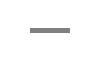
\begin{tikzpicture}[baseline = -0.5ex]
  \draw[line width = 2, color = gray] (0, 0) -- (0.5, 0);
  \end{tikzpicture}  
}

% Directed solid edge
\newcommand{\EDS}{
  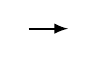
\begin{tikzpicture}[baseline = -0.5ex]
  \draw[->] (0, 0) -- (0.5, 0);
  \end{tikzpicture}  
}

% Directed dotted edge
\newcommand{\EDD}{
  \begin{tikzpicture}[baseline = -0.5ex]
  \draw[->, dotted] (0, 0) -- (0.5, 0);
  \end{tikzpicture}
}

%Análisis léxico
\newcommand{\str}[1]{\textbf{\texttt{#1}}}
\newcommand{\dash}{\text{--}}

%Recuadros
\definecolor{FondoRecuadro}{rgb}{0.90,0.90,1.0}
\makeatletter
\newenvironment{recuadro}{%
  \noindent%
  \begin{lrbox}{\@tempboxa}\begin{minipage}{\columnwidth}}{\end{minipage}\end{lrbox}%
  \colorbox{FondoRecuadro}{\usebox{\@tempboxa}}
}
\makeatother